% =====================================================================
% poc_section.tex  --  new section "Proof-of-Concept Instantiation"
% Paste before the Conclusion, after the section of Improvement 1, or % =====================================================================
% poc_section.tex  --  Proof of Concept of a scaled-down SkeltyMLOps (Person A, Part 6)
% Insert into the main report with:  % =====================================================================
% poc_section.tex  --  Proof of Concept of a scaled-down SkeltyMLOps (Person A, Part 6)
% Insert into the main report with:  % =====================================================================
% poc_section.tex  --  Proof of Concept of a scaled-down SkeltyMLOps (Person A, Part 6)
% Insert into the main report with:  \input{poc_section}
% Required packages in the preamble: booktabs, longtable, array, tikz
% Required TikZ libraries: positioning, arrows.meta, shapes.geometric, fit, backgrounds
% Architecture reference: Daoud et al., Future Generation Computer Systems 185 (2026) 108700.
%
% Source of every number in Section "Results":
%   scenario/logs/20261015T121211Z.md  (single run, 2026-10-15)
%   evidence/10-retrain-issue-7-train.png (accuracy and F1 of issue-7)
%   PROGRESS.md (test counts, cluster description)
% Nothing in this file is estimated. If a new scenario run replaces the log,
% every value in Table~\ref{tab:poc-results} and the timings must be re-read from the new log.
%
% Checked against the paper (FGCS 185, 108700): component names follow Fig. 6 and Table 9;
% Fig. 3 of the paper is the SLR process, so "Figure 3" in task.md is not the architecture figure.
%
% To confirm before submission:
%   (1) the labels sec:poc, fig:poc-architecture, tab:poc-mapping, tab:poc-results do not clash
%       with labels in the main report;
%   (2) \papercite below matches the way the main report cites the paper.
% =====================================================================

% Reference to the paper under study (same definition as in scoring_section.tex).
% Person C: replace with \cite{<bib key of Daoud et al. 2026>} if needed.
\providecommand{\papercite}{[1]}

\section{Proof of Concept: A Scaled-Down SkeltyMLOps}
\label{sec:poc}

\subsection{Goal and Scope}

Daoud et al.~\papercite{} support SkeltyMLOps only with one illustrative ticket lifecycle (Section~5.9 of the paper). Their coverage analysis scores five baseline architectures but not SkeltyMLOps, and the architecture has not been instantiated in a production setting (Sections~5.9 and~5.11); an implementation that orchestrates tools such as MLflow and DVC is reported as ongoing. To check whether its central idea can actually be executed, the group built a small Proof of Concept (PoC) and ran it on a small Kubernetes cluster. The central idea tested is the \emph{feedback loop mediated by a ticket}: a monitoring component detects data drift and raises a ticket, an orchestration component reads the ticket and re-runs the training pipeline, and the serving component loads the new model.

The PoC is deliberately narrow. It answers one question only: \emph{can the drift $\rightarrow$ ticket $\rightarrow$ retrain $\rightarrow$ reload loop run end to end without a manual step, using off-the-shelf tools?} It does not evaluate model quality, scalability, security, cost or the usability of the coordination contracts described in the paper. It is a PoC and must not be read as a production system.

\subsection{Mapping Paper Components to the Implementation}

Table~\ref{tab:poc-mapping} maps the components of the SkeltyMLOps architecture (Fig.~6 and Table~9 of~\papercite{}) to what the group implemented. The \emph{Level} column has three values: \emph{Full} (the capability is implemented with a real tool on the real cluster), \emph{Simplified} (implemented, but with fewer features than in the paper or with several components merged), and \emph{Simulated} (replaced by a stand-in that imitates the behaviour).

{\small
\setlength{\tabcolsep}{4pt}
\begin{longtable}{@{}>{\raggedright\arraybackslash}p{3.7cm} >{\raggedright\arraybackslash}p{6.6cm} >{\raggedright\arraybackslash}p{1.9cm}@{}}
\caption{Mapping from the SkeltyMLOps components to the PoC implementation.}
\label{tab:poc-mapping}\\
\toprule
Paper component & PoC implementation & Level \\
\midrule
\endfirsthead
\toprule
Paper component & PoC implementation & Level \\
\midrule
\endhead
\midrule
\multicolumn{3}{r}{\footnotesize Continued on next page}\\
\endfoot
\bottomrule
\endlastfoot

Data Acquisition & \texttt{acquire.py} generates a synthetic tabular data set (6 numeric features, binary label, 1000 samples, fixed seed 42). The \texttt{shift} parameter moves every feature by \texttt{shift} standard deviations to imitate drift. & Simulated \\
Data Processing \& Feature Engineering & \texttt{process.py} makes a stratified 80/20 train/test split and writes the reference statistics (mean and standard deviation of each feature) used later for drift detection. No feature transformation. & Simplified \\
Data, Feature and Model Storage \& Versioning & Plain files on one NFS-backed PersistentVolumeClaim: \texttt{raw/}, \texttt{features/} and \texttt{models/} directories, one sub-directory per \texttt{run-id}. Each \texttt{manifest.json} stores SHA-256 hashes of the raw, train and test data and of the model; a \texttt{LATEST} file points to the active model. The three storage components of the paper are merged into one; MLflow and DVC are not used. & Simplified \\
Code Storage \& Versioning & A Git repository; each pipeline step runs from a container image with a fixed tag (\texttt{skelty-poc:0.1}). Code is not hashed per run. & Simplified \\
Model Development \& Training & \texttt{train.py} fits a scikit-learn logistic regression and writes \texttt{model.joblib}, \texttt{metrics.json} (accuracy, F1) and \texttt{manifest.json}. & Simplified \\
API Development & A FastAPI service with \texttt{/predict}, \texttt{/model}, \texttt{/reload}, \texttt{/stats}, \texttt{/health} and \texttt{/metrics}. \texttt{/stats} returns the mean and standard deviation of the last 200 valid requests. & Simplified \\
Deployment \& Monitoring & A CronJob (every 5 minutes) compares \texttt{/stats} with the reference statistics and pushes three metrics (\texttt{drift\_detected}, \texttt{drifted\_feature\_count}, \texttt{max\_feature\_zscore}) to a Pushgateway; Prometheus and Grafana display them. Only input drift is monitored. & Simplified \\
Project Management (Plan package): tickets & GitHub Issues with the labels \texttt{retrain}, \texttt{in-progress} and \texttt{done}. The issue body carries a JSON block with the drift description. & Simplified \\
MLOps Process Orchestration (MPO): Execute Pipelines & An Argo Workflows \texttt{WorkflowTemplate} runs \texttt{acquire}, \texttt{process} and \texttt{train} in sequence. & Full \\
MPO: Trigger Retraining & A Python service that polls GitHub every 30 seconds, creates one Argo Workflow per issue, waits for the result, calls \texttt{/reload}, comments on and closes the issue. It does not use BPMN and has no explicit coordination contracts. & Simplified \\
Actors and human hand-offs & Not modelled. The monitor and the orchestrator act through one GitHub account; no human approval step exists. & Simulated \\
\end{longtable}
}

\subsection{PoC Architecture}

Figure~\ref{fig:poc-architecture} shows the components and their interfaces. All pods run in the \texttt{argo} namespace and share one ReadWriteOnce PersistentVolumeClaim.

\begin{figure}[htbp]
\centering
\begin{tikzpicture}[
  font=\scriptsize,
  box/.style={draw, rounded corners=2pt, align=center, minimum width=2.8cm, minimum height=1.0cm, fill=white},
  store/.style={draw, cylinder, shape border rotate=90, aspect=0.25, align=center, minimum width=2.8cm, minimum height=1.1cm, fill=white},
  ext/.style={draw, dashed, rounded corners=2pt, align=center, minimum width=2.8cm, minimum height=1.0cm, fill=white},
  flow/.style={-{Stealth[length=1.8mm]}, thick},
  lab/.style={font=\tiny, fill=white, inner sep=1pt, align=center}
]
% grid: columns x = 0, 4.4, 8.8 ; rows y = 2.5, 0, -2.5, -5
\node[ext]   (client) at (0,0)      {Client\\(traffic generator)};
\node[box]   (serving) at (4.4,0)   {\textbf{Serving}\\FastAPI, \texttt{skelty-serving}};
\node[box]   (drift) at (8.8,0)     {\textbf{Drift monitor}\\CronJob, every 5 min};
\node[box]   (mon) at (6.6,2.6)     {Pushgateway,\\Prometheus, Grafana};
\node[ext]   (issue) at (8.8,-2.6)  {Ticket\\GitHub Issue \texttt{[drift]}};
\node[box]   (orch) at (4.4,-2.6)   {\textbf{Orchestrator}\\polls every 30 s};
\node[store] (store) at (0,-2.6)    {Artifact store\\(NFS PVC)};
\node[box]   (argo) at (0,-5.2)     {\textbf{Argo Workflow}\\acquire $\rightarrow$ process $\rightarrow$ train};

\draw[flow] (client) -- node[lab, above] {\texttt{POST /predict}} (serving);
\draw[flow] (drift) -- node[lab, above] {\texttt{GET /stats},\\\texttt{GET /model}} (serving);
\draw[flow] (serving) -- node[lab, left, pos=0.45] {\texttt{/metrics}} (mon);
\draw[flow] (drift) -- node[lab, right, pos=0.45] {push} (mon);
\draw[flow] (drift) -- node[lab, right] {creates} (issue);
\draw[flow] (orch) -- node[lab, above] {polls, relabels,\\closes} (issue);
\draw[flow] (orch) -- node[lab, right] {\texttt{POST /reload}} (serving);
\draw[flow] (orch) -- node[lab, below, sloped, pos=0.5] {creates Workflow} (argo);
\draw[flow] (argo) -- node[lab, left] {writes} (store);
\draw[flow, dashed] (store) -- node[lab, sloped, above, pos=0.5] {reads model} (serving);
\end{tikzpicture}
\caption{Architecture of the PoC. Solid arrows are calls or writes; the dashed arrow is the serving pod reading the new model from the shared volume after \texttt{/reload}. The drift monitor and the orchestrator also read \texttt{reference\_stats.json} and \texttt{metrics.json} from the same volume (not drawn).}
\label{fig:poc-architecture}
\end{figure}

The feedback loop proceeds as follows.
\begin{enumerate}
  \item Clients send requests to \texttt{/predict}; the serving pod keeps the mean and standard deviation of the last 200 valid requests.
  \item Every 5 minutes the CronJob computes, for each feature, $z = |\mu_{\text{now}} - \mu_{\text{ref}}| / \sigma_{\text{ref}}$ against the reference statistics of the model currently served. \textbf{Drift is declared when at least 3 features have $z > 1.0$ and the window holds at least 100 samples.}
  \item If drift is declared and no issue with the label \texttt{retrain} is open, the CronJob creates an issue whose title starts with \texttt{[drift]} and whose body contains a JSON block (\texttt{type}, \texttt{model\_version}, \texttt{drifted\_features}, \texttt{detected\_at}).
  \item The orchestrator adds the label \texttt{in-progress}, creates a Workflow named \texttt{retrain-issue-<number>} (so a restart cannot create a second one), and waits for it to finish with a 900-second timeout. Its default \texttt{shift} is 1.5, so the retrained model is fitted to the shifted data.
  \item On success it calls \texttt{/reload}, comments with the accuracy and F1 read from \texttt{metrics.json}, adds \texttt{done} and closes the issue. On failure or timeout it comments, removes \texttt{in-progress} and leaves the issue open.
  \item \texttt{/reload} also clears the statistics window, so after a retrain at least 100 new samples must be collected before drift can be reported again; this prevents an endless loop of tickets.
\end{enumerate}

\subsection{Experimental Environment}

The PoC ran on a Kubernetes v1.30.14 cluster with three nodes (one control plane and two workers, containerd runtime) in a home laboratory. The control-plane node has 3.8~GiB of RAM and 3 CPU cores. Argo Workflows v4.1.5 was installed with Helm; Prometheus and Grafana come from an existing kube-prometheus-stack, and a Pushgateway was added for the short-lived CronJob. Artifacts are stored on an NFS export through a manually created PersistentVolume. There is no image registry: images were built on one machine and imported into every node. The data are synthetic and the model is a logistic regression.

\subsection{Verification Scenario}

The scenario script \texttt{scenario/run\_scenario.py} runs five steps in order and records for each step the expectation, the observed result and a pass/fail mark. A step that fails is recorded as failed and is never skipped or edited. The parameters were 200 requests per batch and a shift of 1.5 standard deviations.

\begin{enumerate}
  \item \textbf{Baseline.} Run the Workflow with \texttt{run-id} \texttt{baseline-001} and \texttt{shift} 0, wait for it to succeed, call \texttt{/reload} and check that \texttt{/model} reports \texttt{baseline-001}.
  \item \textbf{No drift on original data.} Send 200 requests drawn from the original distribution and check that \texttt{/stats} shows $n \ge 100$ and that the drift rule is not satisfied.
  \item \textbf{Drift detection.} Send 200 requests shifted by 1.5 standard deviations and wait until the drift rule is satisfied and an issue labelled \texttt{retrain} appears.
  \item \textbf{Automatic retraining.} Wait until the orchestrator closes the issue with the label \texttt{done} and \texttt{/model} reports \texttt{issue-<number>}.
  \item \textbf{No drift after retraining.} Send 200 shifted requests again and check that, against the reference statistics of the new model, the drift rule is not satisfied.
\end{enumerate}

\subsection{Results}

The results below come from one run of the scenario on 2026-10-15 (12:06:20Z to 12:12:11Z, about 5 minutes 51 seconds). Table~\ref{tab:poc-results} is copied from the log file \texttt{scenario/logs/20261015T121211Z.md}; times are UTC.

\begin{table}[htbp]
\centering
\small
\caption{Results of the five-step scenario. Source: \texttt{scenario/logs/20261015T121211Z.md}. $z_{\max}$ is the largest per-feature $z$ value printed in the log for that step.}
\label{tab:poc-results}
\begin{tabular}{@{}>{\centering\arraybackslash}p{0.8cm} >{\raggedright\arraybackslash}p{4.4cm} >{\raggedright\arraybackslash}p{6.4cm} >{\centering\arraybackslash}p{1.2cm}@{}}
\toprule
Step & Expected & Observed (from the log) & Result \\
\midrule
1 & Workflow \emph{Succeeded}; \texttt{/model.run\_id} is \texttt{baseline-001} & Workflow \texttt{baseline-001} \emph{Succeeded} at 12:07:32Z; \texttt{/reload} changed the model from \texttt{issue-6} to \texttt{baseline-001} & Pass \\
2 & $n \ge 100$ and no drift & $n = 200$; no feature above the threshold; $z_{\max} = 0.18$ (feature \texttt{f3}) & Pass \\
3 & Drift visible in \texttt{/stats}; a \texttt{[drift]} issue with label \texttt{retrain} appears & Shifted batch sent at 12:07:53Z; all 6 features drifted; issue \#7 created at 12:10:34Z & Pass \\
4 & Issue closed with label \texttt{done}; \texttt{/model.run\_id} is \texttt{issue-<number>} & Issue \#7 closed at 12:12:01Z with labels \texttt{retrain} and \texttt{done}; \texttt{/model.run\_id} is \texttt{issue-7} & Pass \\
5 & $n \ge 100$ and no drift against the new reference & Model \texttt{issue-7}; $n = 200$; no feature above the threshold; $z_{\max} = 0.13$ (feature \texttt{f0}) & Pass \\
\bottomrule
\end{tabular}
\end{table}

\paragraph{Latency of the loop.} From the log timestamps, the issue was created 2 minutes 41 seconds after the shifted batch was sent, and the issue was closed 1 minute 27 seconds after it was created. The loop from the shifted batch (12:07:53Z) to a closed issue and a reloaded model (12:12:01Z) therefore took about 4 minutes 8 seconds in this run; step~5 confirmed the absence of drift at 12:12:11Z, 4 minutes 18 seconds after the batch. The first part is dominated by the 5-minute period of the CronJob, whose position relative to the batch is a matter of chance; the figure is a single observation and not an average.

\paragraph{Retrained model.} The \texttt{train} step of Workflow \texttt{retrain-issue-7} reported accuracy 0.9150 and F1 0.9163 (Argo UI log, \texttt{evidence/10-retrain-issue-7-train.png}); the project notes record the same two values for \texttt{baseline-001}. The values are identical because the synthetic data are generated with the same seed and the shift translates the whole data set, so the classification problem is only moved; what changes is the decision boundary and the reference statistics. \textbf{Accuracy is therefore not evidence that retraining took place.} The evidence is the new \texttt{run-id} (\texttt{issue-7}), the \texttt{shift=1.5} value written in the log of the \texttt{acquire} step, and the disappearance of drift in step~5.

\paragraph{Other observations.} Five issues (\#3 to \#7) were processed by the orchestrator during development and testing, and all were closed; issues \#5 and \#7 were created by the monitor, the others by hand to test the orchestrator. The Grafana dashboard (\texttt{evidence/16}, \texttt{evidence/17}) shows the model version, the number of predictions and the drift metrics returning to near zero after each retrain. The orchestrator log recorded four polling failures caused by a dropped connection to GitHub; the loop recovered each time and the cause was not determined.

\paragraph{Unit tests.} The pipeline, serving, monitoring, orchestrator and scenario code have 68 pytest tests in total (16, 10, 24, 12 and 6 respectively), all passing on a Windows machine with Python 3.12.8. The serving, monitoring, orchestrator and scenario tests use fake services, so they do not replace the cluster run above.

\subsection{Differences from the Paper and Limitations}

\begin{itemize}
  \item \textbf{Scale and data.} The PoC uses a small synthetic tabular data set, a single simple model and one small cluster. Drift is simulated by shifting the distribution, not observed in real traffic. Nothing here shows how the approach behaves with real data, large models or many pipelines.
  \item \textbf{Orchestration.} The orchestrator is a Python polling loop, not a BPMN-driven engine, and the coordination contracts of the paper are not modelled. The group therefore tested the ticket-driven loop, not the contract mechanism that the paper presents as its main contribution.
  \item \textbf{Ticket lifecycle.} In the paper's scenario (Section~5.9) a Product Owner approves retraining, and the ticket is handed off in turn to the Data, Model, Software and Ops modules, with named artifacts (a new dataset version, a new model version) and a code update of the serving endpoint. In the PoC a single automated Workflow replaces the Data and Model handoffs, no human approves the ticket, and there is no Software handoff because the API does not change.
  \item \textbf{Storage and versioning.} Files on an NFS volume with SHA-256 hashes replace MLflow and DVC, and the data, feature and model storage components are merged. Code is versioned only through Git and image tags.
  \item \textbf{Monitoring.} Only input drift is detected. There are no true labels at run time, so model accuracy in production is not measured. The statistics window lives in the memory of one pod and is lost when the pod restarts. Pushgateway keeps the last pushed value, so the metrics stay frozen if the CronJob stops.
  \item \textbf{Detection delay.} The window holds the last 200 requests, so drift is not reported as soon as the data begin to change: a local measurement (not on the cluster) with 60 shifted requests mixed with 140 original ones gave $z$ values of only 0.3 to 0.6. With a shift of 1.5 standard deviations, roughly more than 134 of the 200 requests must be shifted before the threshold is exceeded.
  \item \textbf{Actors and access.} The monitor and the orchestrator call GitHub with the token of one personal account, so a human action cannot be told apart from an automatic one in the GitHub history. No human approval step exists before retraining.
  \item \textbf{Single run.} The scenario was run once. There is no repetition, no variance and no measurement of failure cases on the cluster (for example, a failing Workflow); these cases are covered only by the unit tests with fake services.
  \item \textbf{Infrastructure.} The control-plane node was short of memory on 2026-10-13 (the API server used about 2.3 to 2.5~GB of 3.8~GB), around the time Argo Workflows was installed. The root cause was not established and a link to that installation is only suspected, and memory use during the scenario run was not recorded.
\end{itemize}

\subsection{Conclusion}

In this single run on a small cluster, the ticket-driven loop worked from drift detection to a reloaded model without a manual step, and all five scenario steps passed. This supports a narrow claim: the loop described in Section~5.9 of the paper can be implemented with Argo Workflows, a small drift check and an issue tracker. It does not show that the full SkeltyMLOps architecture, in particular its coordination contracts and BPMN-based orchestration, works as the paper describes, nor that it scales or improves model quality. These questions remain open and would need real data, repeated runs and a closer implementation of the orchestrator.

% Required packages in the preamble: booktabs, longtable, array, tikz
% Required TikZ libraries: positioning, arrows.meta, shapes.geometric, fit, backgrounds
% Architecture reference: Daoud et al., Future Generation Computer Systems 185 (2026) 108700.
%
% Source of every number in Section "Results":
%   scenario/logs/20261015T121211Z.md  (single run, 2026-10-15)
%   evidence/10-retrain-issue-7-train.png (accuracy and F1 of issue-7)
%   PROGRESS.md (test counts, cluster description)
% Nothing in this file is estimated. If a new scenario run replaces the log,
% every value in Table~\ref{tab:poc-results} and the timings must be re-read from the new log.
%
% Checked against the paper (FGCS 185, 108700): component names follow Fig. 6 and Table 9;
% Fig. 3 of the paper is the SLR process, so "Figure 3" in task.md is not the architecture figure.
%
% To confirm before submission:
%   (1) the labels sec:poc, fig:poc-architecture, tab:poc-mapping, tab:poc-results do not clash
%       with labels in the main report;
%   (2) \papercite below matches the way the main report cites the paper.
% =====================================================================

% Reference to the paper under study (same definition as in scoring_section.tex).
% Person C: replace with \cite{<bib key of Daoud et al. 2026>} if needed.
\providecommand{\papercite}{[1]}

\section{Proof of Concept: A Scaled-Down SkeltyMLOps}
\label{sec:poc}

\subsection{Goal and Scope}

Daoud et al.~\papercite{} support SkeltyMLOps only with one illustrative ticket lifecycle (Section~5.9 of the paper). Their coverage analysis scores five baseline architectures but not SkeltyMLOps, and the architecture has not been instantiated in a production setting (Sections~5.9 and~5.11); an implementation that orchestrates tools such as MLflow and DVC is reported as ongoing. To check whether its central idea can actually be executed, the group built a small Proof of Concept (PoC) and ran it on a small Kubernetes cluster. The central idea tested is the \emph{feedback loop mediated by a ticket}: a monitoring component detects data drift and raises a ticket, an orchestration component reads the ticket and re-runs the training pipeline, and the serving component loads the new model.

The PoC is deliberately narrow. It answers one question only: \emph{can the drift $\rightarrow$ ticket $\rightarrow$ retrain $\rightarrow$ reload loop run end to end without a manual step, using off-the-shelf tools?} It does not evaluate model quality, scalability, security, cost or the usability of the coordination contracts described in the paper. It is a PoC and must not be read as a production system.

\subsection{Mapping Paper Components to the Implementation}

Table~\ref{tab:poc-mapping} maps the components of the SkeltyMLOps architecture (Fig.~6 and Table~9 of~\papercite{}) to what the group implemented. The \emph{Level} column has three values: \emph{Full} (the capability is implemented with a real tool on the real cluster), \emph{Simplified} (implemented, but with fewer features than in the paper or with several components merged), and \emph{Simulated} (replaced by a stand-in that imitates the behaviour).

{\small
\setlength{\tabcolsep}{4pt}
\begin{longtable}{@{}>{\raggedright\arraybackslash}p{3.7cm} >{\raggedright\arraybackslash}p{6.6cm} >{\raggedright\arraybackslash}p{1.9cm}@{}}
\caption{Mapping from the SkeltyMLOps components to the PoC implementation.}
\label{tab:poc-mapping}\\
\toprule
Paper component & PoC implementation & Level \\
\midrule
\endfirsthead
\toprule
Paper component & PoC implementation & Level \\
\midrule
\endhead
\midrule
\multicolumn{3}{r}{\footnotesize Continued on next page}\\
\endfoot
\bottomrule
\endlastfoot

Data Acquisition & \texttt{acquire.py} generates a synthetic tabular data set (6 numeric features, binary label, 1000 samples, fixed seed 42). The \texttt{shift} parameter moves every feature by \texttt{shift} standard deviations to imitate drift. & Simulated \\
Data Processing \& Feature Engineering & \texttt{process.py} makes a stratified 80/20 train/test split and writes the reference statistics (mean and standard deviation of each feature) used later for drift detection. No feature transformation. & Simplified \\
Data, Feature and Model Storage \& Versioning & Plain files on one NFS-backed PersistentVolumeClaim: \texttt{raw/}, \texttt{features/} and \texttt{models/} directories, one sub-directory per \texttt{run-id}. Each \texttt{manifest.json} stores SHA-256 hashes of the raw, train and test data and of the model; a \texttt{LATEST} file points to the active model. The three storage components of the paper are merged into one; MLflow and DVC are not used. & Simplified \\
Code Storage \& Versioning & A Git repository; each pipeline step runs from a container image with a fixed tag (\texttt{skelty-poc:0.1}). Code is not hashed per run. & Simplified \\
Model Development \& Training & \texttt{train.py} fits a scikit-learn logistic regression and writes \texttt{model.joblib}, \texttt{metrics.json} (accuracy, F1) and \texttt{manifest.json}. & Simplified \\
API Development & A FastAPI service with \texttt{/predict}, \texttt{/model}, \texttt{/reload}, \texttt{/stats}, \texttt{/health} and \texttt{/metrics}. \texttt{/stats} returns the mean and standard deviation of the last 200 valid requests. & Simplified \\
Deployment \& Monitoring & A CronJob (every 5 minutes) compares \texttt{/stats} with the reference statistics and pushes three metrics (\texttt{drift\_detected}, \texttt{drifted\_feature\_count}, \texttt{max\_feature\_zscore}) to a Pushgateway; Prometheus and Grafana display them. Only input drift is monitored. & Simplified \\
Project Management (Plan package): tickets & GitHub Issues with the labels \texttt{retrain}, \texttt{in-progress} and \texttt{done}. The issue body carries a JSON block with the drift description. & Simplified \\
MLOps Process Orchestration (MPO): Execute Pipelines & An Argo Workflows \texttt{WorkflowTemplate} runs \texttt{acquire}, \texttt{process} and \texttt{train} in sequence. & Full \\
MPO: Trigger Retraining & A Python service that polls GitHub every 30 seconds, creates one Argo Workflow per issue, waits for the result, calls \texttt{/reload}, comments on and closes the issue. It does not use BPMN and has no explicit coordination contracts. & Simplified \\
Actors and human hand-offs & Not modelled. The monitor and the orchestrator act through one GitHub account; no human approval step exists. & Simulated \\
\end{longtable}
}

\subsection{PoC Architecture}

Figure~\ref{fig:poc-architecture} shows the components and their interfaces. All pods run in the \texttt{argo} namespace and share one ReadWriteOnce PersistentVolumeClaim.

\begin{figure}[htbp]
\centering
\begin{tikzpicture}[
  font=\scriptsize,
  box/.style={draw, rounded corners=2pt, align=center, minimum width=2.8cm, minimum height=1.0cm, fill=white},
  store/.style={draw, cylinder, shape border rotate=90, aspect=0.25, align=center, minimum width=2.8cm, minimum height=1.1cm, fill=white},
  ext/.style={draw, dashed, rounded corners=2pt, align=center, minimum width=2.8cm, minimum height=1.0cm, fill=white},
  flow/.style={-{Stealth[length=1.8mm]}, thick},
  lab/.style={font=\tiny, fill=white, inner sep=1pt, align=center}
]
% grid: columns x = 0, 4.4, 8.8 ; rows y = 2.5, 0, -2.5, -5
\node[ext]   (client) at (0,0)      {Client\\(traffic generator)};
\node[box]   (serving) at (4.4,0)   {\textbf{Serving}\\FastAPI, \texttt{skelty-serving}};
\node[box]   (drift) at (8.8,0)     {\textbf{Drift monitor}\\CronJob, every 5 min};
\node[box]   (mon) at (6.6,2.6)     {Pushgateway,\\Prometheus, Grafana};
\node[ext]   (issue) at (8.8,-2.6)  {Ticket\\GitHub Issue \texttt{[drift]}};
\node[box]   (orch) at (4.4,-2.6)   {\textbf{Orchestrator}\\polls every 30 s};
\node[store] (store) at (0,-2.6)    {Artifact store\\(NFS PVC)};
\node[box]   (argo) at (0,-5.2)     {\textbf{Argo Workflow}\\acquire $\rightarrow$ process $\rightarrow$ train};

\draw[flow] (client) -- node[lab, above] {\texttt{POST /predict}} (serving);
\draw[flow] (drift) -- node[lab, above] {\texttt{GET /stats},\\\texttt{GET /model}} (serving);
\draw[flow] (serving) -- node[lab, left, pos=0.45] {\texttt{/metrics}} (mon);
\draw[flow] (drift) -- node[lab, right, pos=0.45] {push} (mon);
\draw[flow] (drift) -- node[lab, right] {creates} (issue);
\draw[flow] (orch) -- node[lab, above] {polls, relabels,\\closes} (issue);
\draw[flow] (orch) -- node[lab, right] {\texttt{POST /reload}} (serving);
\draw[flow] (orch) -- node[lab, below, sloped, pos=0.5] {creates Workflow} (argo);
\draw[flow] (argo) -- node[lab, left] {writes} (store);
\draw[flow, dashed] (store) -- node[lab, sloped, above, pos=0.5] {reads model} (serving);
\end{tikzpicture}
\caption{Architecture of the PoC. Solid arrows are calls or writes; the dashed arrow is the serving pod reading the new model from the shared volume after \texttt{/reload}. The drift monitor and the orchestrator also read \texttt{reference\_stats.json} and \texttt{metrics.json} from the same volume (not drawn).}
\label{fig:poc-architecture}
\end{figure}

The feedback loop proceeds as follows.
\begin{enumerate}
  \item Clients send requests to \texttt{/predict}; the serving pod keeps the mean and standard deviation of the last 200 valid requests.
  \item Every 5 minutes the CronJob computes, for each feature, $z = |\mu_{\text{now}} - \mu_{\text{ref}}| / \sigma_{\text{ref}}$ against the reference statistics of the model currently served. \textbf{Drift is declared when at least 3 features have $z > 1.0$ and the window holds at least 100 samples.}
  \item If drift is declared and no issue with the label \texttt{retrain} is open, the CronJob creates an issue whose title starts with \texttt{[drift]} and whose body contains a JSON block (\texttt{type}, \texttt{model\_version}, \texttt{drifted\_features}, \texttt{detected\_at}).
  \item The orchestrator adds the label \texttt{in-progress}, creates a Workflow named \texttt{retrain-issue-<number>} (so a restart cannot create a second one), and waits for it to finish with a 900-second timeout. Its default \texttt{shift} is 1.5, so the retrained model is fitted to the shifted data.
  \item On success it calls \texttt{/reload}, comments with the accuracy and F1 read from \texttt{metrics.json}, adds \texttt{done} and closes the issue. On failure or timeout it comments, removes \texttt{in-progress} and leaves the issue open.
  \item \texttt{/reload} also clears the statistics window, so after a retrain at least 100 new samples must be collected before drift can be reported again; this prevents an endless loop of tickets.
\end{enumerate}

\subsection{Experimental Environment}

The PoC ran on a Kubernetes v1.30.14 cluster with three nodes (one control plane and two workers, containerd runtime) in a home laboratory. The control-plane node has 3.8~GiB of RAM and 3 CPU cores. Argo Workflows v4.1.5 was installed with Helm; Prometheus and Grafana come from an existing kube-prometheus-stack, and a Pushgateway was added for the short-lived CronJob. Artifacts are stored on an NFS export through a manually created PersistentVolume. There is no image registry: images were built on one machine and imported into every node. The data are synthetic and the model is a logistic regression.

\subsection{Verification Scenario}

The scenario script \texttt{scenario/run\_scenario.py} runs five steps in order and records for each step the expectation, the observed result and a pass/fail mark. A step that fails is recorded as failed and is never skipped or edited. The parameters were 200 requests per batch and a shift of 1.5 standard deviations.

\begin{enumerate}
  \item \textbf{Baseline.} Run the Workflow with \texttt{run-id} \texttt{baseline-001} and \texttt{shift} 0, wait for it to succeed, call \texttt{/reload} and check that \texttt{/model} reports \texttt{baseline-001}.
  \item \textbf{No drift on original data.} Send 200 requests drawn from the original distribution and check that \texttt{/stats} shows $n \ge 100$ and that the drift rule is not satisfied.
  \item \textbf{Drift detection.} Send 200 requests shifted by 1.5 standard deviations and wait until the drift rule is satisfied and an issue labelled \texttt{retrain} appears.
  \item \textbf{Automatic retraining.} Wait until the orchestrator closes the issue with the label \texttt{done} and \texttt{/model} reports \texttt{issue-<number>}.
  \item \textbf{No drift after retraining.} Send 200 shifted requests again and check that, against the reference statistics of the new model, the drift rule is not satisfied.
\end{enumerate}

\subsection{Results}

The results below come from one run of the scenario on 2026-10-15 (12:06:20Z to 12:12:11Z, about 5 minutes 51 seconds). Table~\ref{tab:poc-results} is copied from the log file \texttt{scenario/logs/20261015T121211Z.md}; times are UTC.

\begin{table}[htbp]
\centering
\small
\caption{Results of the five-step scenario. Source: \texttt{scenario/logs/20261015T121211Z.md}. $z_{\max}$ is the largest per-feature $z$ value printed in the log for that step.}
\label{tab:poc-results}
\begin{tabular}{@{}>{\centering\arraybackslash}p{0.8cm} >{\raggedright\arraybackslash}p{4.4cm} >{\raggedright\arraybackslash}p{6.4cm} >{\centering\arraybackslash}p{1.2cm}@{}}
\toprule
Step & Expected & Observed (from the log) & Result \\
\midrule
1 & Workflow \emph{Succeeded}; \texttt{/model.run\_id} is \texttt{baseline-001} & Workflow \texttt{baseline-001} \emph{Succeeded} at 12:07:32Z; \texttt{/reload} changed the model from \texttt{issue-6} to \texttt{baseline-001} & Pass \\
2 & $n \ge 100$ and no drift & $n = 200$; no feature above the threshold; $z_{\max} = 0.18$ (feature \texttt{f3}) & Pass \\
3 & Drift visible in \texttt{/stats}; a \texttt{[drift]} issue with label \texttt{retrain} appears & Shifted batch sent at 12:07:53Z; all 6 features drifted; issue \#7 created at 12:10:34Z & Pass \\
4 & Issue closed with label \texttt{done}; \texttt{/model.run\_id} is \texttt{issue-<number>} & Issue \#7 closed at 12:12:01Z with labels \texttt{retrain} and \texttt{done}; \texttt{/model.run\_id} is \texttt{issue-7} & Pass \\
5 & $n \ge 100$ and no drift against the new reference & Model \texttt{issue-7}; $n = 200$; no feature above the threshold; $z_{\max} = 0.13$ (feature \texttt{f0}) & Pass \\
\bottomrule
\end{tabular}
\end{table}

\paragraph{Latency of the loop.} From the log timestamps, the issue was created 2 minutes 41 seconds after the shifted batch was sent, and the issue was closed 1 minute 27 seconds after it was created. The loop from the shifted batch (12:07:53Z) to a closed issue and a reloaded model (12:12:01Z) therefore took about 4 minutes 8 seconds in this run; step~5 confirmed the absence of drift at 12:12:11Z, 4 minutes 18 seconds after the batch. The first part is dominated by the 5-minute period of the CronJob, whose position relative to the batch is a matter of chance; the figure is a single observation and not an average.

\paragraph{Retrained model.} The \texttt{train} step of Workflow \texttt{retrain-issue-7} reported accuracy 0.9150 and F1 0.9163 (Argo UI log, \texttt{evidence/10-retrain-issue-7-train.png}); the project notes record the same two values for \texttt{baseline-001}. The values are identical because the synthetic data are generated with the same seed and the shift translates the whole data set, so the classification problem is only moved; what changes is the decision boundary and the reference statistics. \textbf{Accuracy is therefore not evidence that retraining took place.} The evidence is the new \texttt{run-id} (\texttt{issue-7}), the \texttt{shift=1.5} value written in the log of the \texttt{acquire} step, and the disappearance of drift in step~5.

\paragraph{Other observations.} Five issues (\#3 to \#7) were processed by the orchestrator during development and testing, and all were closed; issues \#5 and \#7 were created by the monitor, the others by hand to test the orchestrator. The Grafana dashboard (\texttt{evidence/16}, \texttt{evidence/17}) shows the model version, the number of predictions and the drift metrics returning to near zero after each retrain. The orchestrator log recorded four polling failures caused by a dropped connection to GitHub; the loop recovered each time and the cause was not determined.

\paragraph{Unit tests.} The pipeline, serving, monitoring, orchestrator and scenario code have 68 pytest tests in total (16, 10, 24, 12 and 6 respectively), all passing on a Windows machine with Python 3.12.8. The serving, monitoring, orchestrator and scenario tests use fake services, so they do not replace the cluster run above.

\subsection{Differences from the Paper and Limitations}

\begin{itemize}
  \item \textbf{Scale and data.} The PoC uses a small synthetic tabular data set, a single simple model and one small cluster. Drift is simulated by shifting the distribution, not observed in real traffic. Nothing here shows how the approach behaves with real data, large models or many pipelines.
  \item \textbf{Orchestration.} The orchestrator is a Python polling loop, not a BPMN-driven engine, and the coordination contracts of the paper are not modelled. The group therefore tested the ticket-driven loop, not the contract mechanism that the paper presents as its main contribution.
  \item \textbf{Ticket lifecycle.} In the paper's scenario (Section~5.9) a Product Owner approves retraining, and the ticket is handed off in turn to the Data, Model, Software and Ops modules, with named artifacts (a new dataset version, a new model version) and a code update of the serving endpoint. In the PoC a single automated Workflow replaces the Data and Model handoffs, no human approves the ticket, and there is no Software handoff because the API does not change.
  \item \textbf{Storage and versioning.} Files on an NFS volume with SHA-256 hashes replace MLflow and DVC, and the data, feature and model storage components are merged. Code is versioned only through Git and image tags.
  \item \textbf{Monitoring.} Only input drift is detected. There are no true labels at run time, so model accuracy in production is not measured. The statistics window lives in the memory of one pod and is lost when the pod restarts. Pushgateway keeps the last pushed value, so the metrics stay frozen if the CronJob stops.
  \item \textbf{Detection delay.} The window holds the last 200 requests, so drift is not reported as soon as the data begin to change: a local measurement (not on the cluster) with 60 shifted requests mixed with 140 original ones gave $z$ values of only 0.3 to 0.6. With a shift of 1.5 standard deviations, roughly more than 134 of the 200 requests must be shifted before the threshold is exceeded.
  \item \textbf{Actors and access.} The monitor and the orchestrator call GitHub with the token of one personal account, so a human action cannot be told apart from an automatic one in the GitHub history. No human approval step exists before retraining.
  \item \textbf{Single run.} The scenario was run once. There is no repetition, no variance and no measurement of failure cases on the cluster (for example, a failing Workflow); these cases are covered only by the unit tests with fake services.
  \item \textbf{Infrastructure.} The control-plane node was short of memory on 2026-10-13 (the API server used about 2.3 to 2.5~GB of 3.8~GB), around the time Argo Workflows was installed. The root cause was not established and a link to that installation is only suspected, and memory use during the scenario run was not recorded.
\end{itemize}

\subsection{Conclusion}

In this single run on a small cluster, the ticket-driven loop worked from drift detection to a reloaded model without a manual step, and all five scenario steps passed. This supports a narrow claim: the loop described in Section~5.9 of the paper can be implemented with Argo Workflows, a small drift check and an issue tracker. It does not show that the full SkeltyMLOps architecture, in particular its coordination contracts and BPMN-based orchestration, works as the paper describes, nor that it scales or improves model quality. These questions remain open and would need real data, repeated runs and a closer implementation of the orchestrator.

% Required packages in the preamble: booktabs, longtable, array, tikz
% Required TikZ libraries: positioning, arrows.meta, shapes.geometric, fit, backgrounds
% Architecture reference: Daoud et al., Future Generation Computer Systems 185 (2026) 108700.
%
% Source of every number in Section "Results":
%   scenario/logs/20261015T121211Z.md  (single run, 2026-10-15)
%   evidence/10-retrain-issue-7-train.png (accuracy and F1 of issue-7)
%   PROGRESS.md (test counts, cluster description)
% Nothing in this file is estimated. If a new scenario run replaces the log,
% every value in Table~\ref{tab:poc-results} and the timings must be re-read from the new log.
%
% Checked against the paper (FGCS 185, 108700): component names follow Fig. 6 and Table 9;
% Fig. 3 of the paper is the SLR process, so "Figure 3" in task.md is not the architecture figure.
%
% To confirm before submission:
%   (1) the labels sec:poc, fig:poc-architecture, tab:poc-mapping, tab:poc-results do not clash
%       with labels in the main report;
%   (2) \papercite below matches the way the main report cites the paper.
% =====================================================================

% Reference to the paper under study (same definition as in scoring_section.tex).
% Person C: replace with \cite{<bib key of Daoud et al. 2026>} if needed.
\providecommand{\papercite}{[1]}

\section{Proof of Concept: A Scaled-Down SkeltyMLOps}
\label{sec:poc}

\subsection{Goal and Scope}

Daoud et al.~\papercite{} support SkeltyMLOps only with one illustrative ticket lifecycle (Section~5.9 of the paper). Their coverage analysis scores five baseline architectures but not SkeltyMLOps, and the architecture has not been instantiated in a production setting (Sections~5.9 and~5.11); an implementation that orchestrates tools such as MLflow and DVC is reported as ongoing. To check whether its central idea can actually be executed, the group built a small Proof of Concept (PoC) and ran it on a small Kubernetes cluster. The central idea tested is the \emph{feedback loop mediated by a ticket}: a monitoring component detects data drift and raises a ticket, an orchestration component reads the ticket and re-runs the training pipeline, and the serving component loads the new model.

The PoC is deliberately narrow. It answers one question only: \emph{can the drift $\rightarrow$ ticket $\rightarrow$ retrain $\rightarrow$ reload loop run end to end without a manual step, using off-the-shelf tools?} It does not evaluate model quality, scalability, security, cost or the usability of the coordination contracts described in the paper. It is a PoC and must not be read as a production system.

\subsection{Mapping Paper Components to the Implementation}

Table~\ref{tab:poc-mapping} maps the components of the SkeltyMLOps architecture (Fig.~6 and Table~9 of~\papercite{}) to what the group implemented. The \emph{Level} column has three values: \emph{Full} (the capability is implemented with a real tool on the real cluster), \emph{Simplified} (implemented, but with fewer features than in the paper or with several components merged), and \emph{Simulated} (replaced by a stand-in that imitates the behaviour).

{\small
\setlength{\tabcolsep}{4pt}
\begin{longtable}{@{}>{\raggedright\arraybackslash}p{3.7cm} >{\raggedright\arraybackslash}p{6.6cm} >{\raggedright\arraybackslash}p{1.9cm}@{}}
\caption{Mapping from the SkeltyMLOps components to the PoC implementation.}
\label{tab:poc-mapping}\\
\toprule
Paper component & PoC implementation & Level \\
\midrule
\endfirsthead
\toprule
Paper component & PoC implementation & Level \\
\midrule
\endhead
\midrule
\multicolumn{3}{r}{\footnotesize Continued on next page}\\
\endfoot
\bottomrule
\endlastfoot

Data Acquisition & \texttt{acquire.py} generates a synthetic tabular data set (6 numeric features, binary label, 1000 samples, fixed seed 42). The \texttt{shift} parameter moves every feature by \texttt{shift} standard deviations to imitate drift. & Simulated \\
Data Processing \& Feature Engineering & \texttt{process.py} makes a stratified 80/20 train/test split and writes the reference statistics (mean and standard deviation of each feature) used later for drift detection. No feature transformation. & Simplified \\
Data, Feature and Model Storage \& Versioning & Plain files on one NFS-backed PersistentVolumeClaim: \texttt{raw/}, \texttt{features/} and \texttt{models/} directories, one sub-directory per \texttt{run-id}. Each \texttt{manifest.json} stores SHA-256 hashes of the raw, train and test data and of the model; a \texttt{LATEST} file points to the active model. The three storage components of the paper are merged into one; MLflow and DVC are not used. & Simplified \\
Code Storage \& Versioning & A Git repository; each pipeline step runs from a container image with a fixed tag (\texttt{skelty-poc:0.1}). Code is not hashed per run. & Simplified \\
Model Development \& Training & \texttt{train.py} fits a scikit-learn logistic regression and writes \texttt{model.joblib}, \texttt{metrics.json} (accuracy, F1) and \texttt{manifest.json}. & Simplified \\
API Development & A FastAPI service with \texttt{/predict}, \texttt{/model}, \texttt{/reload}, \texttt{/stats}, \texttt{/health} and \texttt{/metrics}. \texttt{/stats} returns the mean and standard deviation of the last 200 valid requests. & Simplified \\
Deployment \& Monitoring & A CronJob (every 5 minutes) compares \texttt{/stats} with the reference statistics and pushes three metrics (\texttt{drift\_detected}, \texttt{drifted\_feature\_count}, \texttt{max\_feature\_zscore}) to a Pushgateway; Prometheus and Grafana display them. Only input drift is monitored. & Simplified \\
Project Management (Plan package): tickets & GitHub Issues with the labels \texttt{retrain}, \texttt{in-progress} and \texttt{done}. The issue body carries a JSON block with the drift description. & Simplified \\
MLOps Process Orchestration (MPO): Execute Pipelines & An Argo Workflows \texttt{WorkflowTemplate} runs \texttt{acquire}, \texttt{process} and \texttt{train} in sequence. & Full \\
MPO: Trigger Retraining & A Python service that polls GitHub every 30 seconds, creates one Argo Workflow per issue, waits for the result, calls \texttt{/reload}, comments on and closes the issue. It does not use BPMN and has no explicit coordination contracts. & Simplified \\
Actors and human hand-offs & Not modelled. The monitor and the orchestrator act through one GitHub account; no human approval step exists. & Simulated \\
\end{longtable}
}

\subsection{PoC Architecture}

Figure~\ref{fig:poc-architecture} shows the components and their interfaces. All pods run in the \texttt{argo} namespace and share one ReadWriteOnce PersistentVolumeClaim.

\begin{figure}[htbp]
\centering
\begin{tikzpicture}[
  font=\scriptsize,
  box/.style={draw, rounded corners=2pt, align=center, minimum width=2.8cm, minimum height=1.0cm, fill=white},
  store/.style={draw, cylinder, shape border rotate=90, aspect=0.25, align=center, minimum width=2.8cm, minimum height=1.1cm, fill=white},
  ext/.style={draw, dashed, rounded corners=2pt, align=center, minimum width=2.8cm, minimum height=1.0cm, fill=white},
  flow/.style={-{Stealth[length=1.8mm]}, thick},
  lab/.style={font=\tiny, fill=white, inner sep=1pt, align=center}
]
% grid: columns x = 0, 4.4, 8.8 ; rows y = 2.5, 0, -2.5, -5
\node[ext]   (client) at (0,0)      {Client\\(traffic generator)};
\node[box]   (serving) at (4.4,0)   {\textbf{Serving}\\FastAPI, \texttt{skelty-serving}};
\node[box]   (drift) at (8.8,0)     {\textbf{Drift monitor}\\CronJob, every 5 min};
\node[box]   (mon) at (6.6,2.6)     {Pushgateway,\\Prometheus, Grafana};
\node[ext]   (issue) at (8.8,-2.6)  {Ticket\\GitHub Issue \texttt{[drift]}};
\node[box]   (orch) at (4.4,-2.6)   {\textbf{Orchestrator}\\polls every 30 s};
\node[store] (store) at (0,-2.6)    {Artifact store\\(NFS PVC)};
\node[box]   (argo) at (0,-5.2)     {\textbf{Argo Workflow}\\acquire $\rightarrow$ process $\rightarrow$ train};

\draw[flow] (client) -- node[lab, above] {\texttt{POST /predict}} (serving);
\draw[flow] (drift) -- node[lab, above] {\texttt{GET /stats},\\\texttt{GET /model}} (serving);
\draw[flow] (serving) -- node[lab, left, pos=0.45] {\texttt{/metrics}} (mon);
\draw[flow] (drift) -- node[lab, right, pos=0.45] {push} (mon);
\draw[flow] (drift) -- node[lab, right] {creates} (issue);
\draw[flow] (orch) -- node[lab, above] {polls, relabels,\\closes} (issue);
\draw[flow] (orch) -- node[lab, right] {\texttt{POST /reload}} (serving);
\draw[flow] (orch) -- node[lab, below, sloped, pos=0.5] {creates Workflow} (argo);
\draw[flow] (argo) -- node[lab, left] {writes} (store);
\draw[flow, dashed] (store) -- node[lab, sloped, above, pos=0.5] {reads model} (serving);
\end{tikzpicture}
\caption{Architecture of the PoC. Solid arrows are calls or writes; the dashed arrow is the serving pod reading the new model from the shared volume after \texttt{/reload}. The drift monitor and the orchestrator also read \texttt{reference\_stats.json} and \texttt{metrics.json} from the same volume (not drawn).}
\label{fig:poc-architecture}
\end{figure}

The feedback loop proceeds as follows.
\begin{enumerate}
  \item Clients send requests to \texttt{/predict}; the serving pod keeps the mean and standard deviation of the last 200 valid requests.
  \item Every 5 minutes the CronJob computes, for each feature, $z = |\mu_{\text{now}} - \mu_{\text{ref}}| / \sigma_{\text{ref}}$ against the reference statistics of the model currently served. \textbf{Drift is declared when at least 3 features have $z > 1.0$ and the window holds at least 100 samples.}
  \item If drift is declared and no issue with the label \texttt{retrain} is open, the CronJob creates an issue whose title starts with \texttt{[drift]} and whose body contains a JSON block (\texttt{type}, \texttt{model\_version}, \texttt{drifted\_features}, \texttt{detected\_at}).
  \item The orchestrator adds the label \texttt{in-progress}, creates a Workflow named \texttt{retrain-issue-<number>} (so a restart cannot create a second one), and waits for it to finish with a 900-second timeout. Its default \texttt{shift} is 1.5, so the retrained model is fitted to the shifted data.
  \item On success it calls \texttt{/reload}, comments with the accuracy and F1 read from \texttt{metrics.json}, adds \texttt{done} and closes the issue. On failure or timeout it comments, removes \texttt{in-progress} and leaves the issue open.
  \item \texttt{/reload} also clears the statistics window, so after a retrain at least 100 new samples must be collected before drift can be reported again; this prevents an endless loop of tickets.
\end{enumerate}

\subsection{Experimental Environment}

The PoC ran on a Kubernetes v1.30.14 cluster with three nodes (one control plane and two workers, containerd runtime) in a home laboratory. The control-plane node has 3.8~GiB of RAM and 3 CPU cores. Argo Workflows v4.1.5 was installed with Helm; Prometheus and Grafana come from an existing kube-prometheus-stack, and a Pushgateway was added for the short-lived CronJob. Artifacts are stored on an NFS export through a manually created PersistentVolume. There is no image registry: images were built on one machine and imported into every node. The data are synthetic and the model is a logistic regression.

\subsection{Verification Scenario}

The scenario script \texttt{scenario/run\_scenario.py} runs five steps in order and records for each step the expectation, the observed result and a pass/fail mark. A step that fails is recorded as failed and is never skipped or edited. The parameters were 200 requests per batch and a shift of 1.5 standard deviations.

\begin{enumerate}
  \item \textbf{Baseline.} Run the Workflow with \texttt{run-id} \texttt{baseline-001} and \texttt{shift} 0, wait for it to succeed, call \texttt{/reload} and check that \texttt{/model} reports \texttt{baseline-001}.
  \item \textbf{No drift on original data.} Send 200 requests drawn from the original distribution and check that \texttt{/stats} shows $n \ge 100$ and that the drift rule is not satisfied.
  \item \textbf{Drift detection.} Send 200 requests shifted by 1.5 standard deviations and wait until the drift rule is satisfied and an issue labelled \texttt{retrain} appears.
  \item \textbf{Automatic retraining.} Wait until the orchestrator closes the issue with the label \texttt{done} and \texttt{/model} reports \texttt{issue-<number>}.
  \item \textbf{No drift after retraining.} Send 200 shifted requests again and check that, against the reference statistics of the new model, the drift rule is not satisfied.
\end{enumerate}

\subsection{Results}

The results below come from one run of the scenario on 2026-10-15 (12:06:20Z to 12:12:11Z, about 5 minutes 51 seconds). Table~\ref{tab:poc-results} is copied from the log file \texttt{scenario/logs/20261015T121211Z.md}; times are UTC.

\begin{table}[htbp]
\centering
\small
\caption{Results of the five-step scenario. Source: \texttt{scenario/logs/20261015T121211Z.md}. $z_{\max}$ is the largest per-feature $z$ value printed in the log for that step.}
\label{tab:poc-results}
\begin{tabular}{@{}>{\centering\arraybackslash}p{0.8cm} >{\raggedright\arraybackslash}p{4.4cm} >{\raggedright\arraybackslash}p{6.4cm} >{\centering\arraybackslash}p{1.2cm}@{}}
\toprule
Step & Expected & Observed (from the log) & Result \\
\midrule
1 & Workflow \emph{Succeeded}; \texttt{/model.run\_id} is \texttt{baseline-001} & Workflow \texttt{baseline-001} \emph{Succeeded} at 12:07:32Z; \texttt{/reload} changed the model from \texttt{issue-6} to \texttt{baseline-001} & Pass \\
2 & $n \ge 100$ and no drift & $n = 200$; no feature above the threshold; $z_{\max} = 0.18$ (feature \texttt{f3}) & Pass \\
3 & Drift visible in \texttt{/stats}; a \texttt{[drift]} issue with label \texttt{retrain} appears & Shifted batch sent at 12:07:53Z; all 6 features drifted; issue \#7 created at 12:10:34Z & Pass \\
4 & Issue closed with label \texttt{done}; \texttt{/model.run\_id} is \texttt{issue-<number>} & Issue \#7 closed at 12:12:01Z with labels \texttt{retrain} and \texttt{done}; \texttt{/model.run\_id} is \texttt{issue-7} & Pass \\
5 & $n \ge 100$ and no drift against the new reference & Model \texttt{issue-7}; $n = 200$; no feature above the threshold; $z_{\max} = 0.13$ (feature \texttt{f0}) & Pass \\
\bottomrule
\end{tabular}
\end{table}

\paragraph{Latency of the loop.} From the log timestamps, the issue was created 2 minutes 41 seconds after the shifted batch was sent, and the issue was closed 1 minute 27 seconds after it was created. The loop from the shifted batch (12:07:53Z) to a closed issue and a reloaded model (12:12:01Z) therefore took about 4 minutes 8 seconds in this run; step~5 confirmed the absence of drift at 12:12:11Z, 4 minutes 18 seconds after the batch. The first part is dominated by the 5-minute period of the CronJob, whose position relative to the batch is a matter of chance; the figure is a single observation and not an average.

\paragraph{Retrained model.} The \texttt{train} step of Workflow \texttt{retrain-issue-7} reported accuracy 0.9150 and F1 0.9163 (Argo UI log, \texttt{evidence/10-retrain-issue-7-train.png}); the project notes record the same two values for \texttt{baseline-001}. The values are identical because the synthetic data are generated with the same seed and the shift translates the whole data set, so the classification problem is only moved; what changes is the decision boundary and the reference statistics. \textbf{Accuracy is therefore not evidence that retraining took place.} The evidence is the new \texttt{run-id} (\texttt{issue-7}), the \texttt{shift=1.5} value written in the log of the \texttt{acquire} step, and the disappearance of drift in step~5.

\paragraph{Other observations.} Five issues (\#3 to \#7) were processed by the orchestrator during development and testing, and all were closed; issues \#5 and \#7 were created by the monitor, the others by hand to test the orchestrator. The Grafana dashboard (\texttt{evidence/16}, \texttt{evidence/17}) shows the model version, the number of predictions and the drift metrics returning to near zero after each retrain. The orchestrator log recorded four polling failures caused by a dropped connection to GitHub; the loop recovered each time and the cause was not determined.

\paragraph{Unit tests.} The pipeline, serving, monitoring, orchestrator and scenario code have 68 pytest tests in total (16, 10, 24, 12 and 6 respectively), all passing on a Windows machine with Python 3.12.8. The serving, monitoring, orchestrator and scenario tests use fake services, so they do not replace the cluster run above.

\subsection{Differences from the Paper and Limitations}

\begin{itemize}
  \item \textbf{Scale and data.} The PoC uses a small synthetic tabular data set, a single simple model and one small cluster. Drift is simulated by shifting the distribution, not observed in real traffic. Nothing here shows how the approach behaves with real data, large models or many pipelines.
  \item \textbf{Orchestration.} The orchestrator is a Python polling loop, not a BPMN-driven engine, and the coordination contracts of the paper are not modelled. The group therefore tested the ticket-driven loop, not the contract mechanism that the paper presents as its main contribution.
  \item \textbf{Ticket lifecycle.} In the paper's scenario (Section~5.9) a Product Owner approves retraining, and the ticket is handed off in turn to the Data, Model, Software and Ops modules, with named artifacts (a new dataset version, a new model version) and a code update of the serving endpoint. In the PoC a single automated Workflow replaces the Data and Model handoffs, no human approves the ticket, and there is no Software handoff because the API does not change.
  \item \textbf{Storage and versioning.} Files on an NFS volume with SHA-256 hashes replace MLflow and DVC, and the data, feature and model storage components are merged. Code is versioned only through Git and image tags.
  \item \textbf{Monitoring.} Only input drift is detected. There are no true labels at run time, so model accuracy in production is not measured. The statistics window lives in the memory of one pod and is lost when the pod restarts. Pushgateway keeps the last pushed value, so the metrics stay frozen if the CronJob stops.
  \item \textbf{Detection delay.} The window holds the last 200 requests, so drift is not reported as soon as the data begin to change: a local measurement (not on the cluster) with 60 shifted requests mixed with 140 original ones gave $z$ values of only 0.3 to 0.6. With a shift of 1.5 standard deviations, roughly more than 134 of the 200 requests must be shifted before the threshold is exceeded.
  \item \textbf{Actors and access.} The monitor and the orchestrator call GitHub with the token of one personal account, so a human action cannot be told apart from an automatic one in the GitHub history. No human approval step exists before retraining.
  \item \textbf{Single run.} The scenario was run once. There is no repetition, no variance and no measurement of failure cases on the cluster (for example, a failing Workflow); these cases are covered only by the unit tests with fake services.
  \item \textbf{Infrastructure.} The control-plane node was short of memory on 2026-10-13 (the API server used about 2.3 to 2.5~GB of 3.8~GB), around the time Argo Workflows was installed. The root cause was not established and a link to that installation is only suspected, and memory use during the scenario run was not recorded.
\end{itemize}

\subsection{Conclusion}

In this single run on a small cluster, the ticket-driven loop worked from drift detection to a reloaded model without a manual step, and all five scenario steps passed. This supports a narrow claim: the loop described in Section~5.9 of the paper can be implemented with Argo Workflows, a small drift check and an issue tracker. It does not show that the full SkeltyMLOps architecture, in particular its coordination contracts and BPMN-based orchestration, works as the paper describes, nor that it scales or improves model quality. These questions remain open and would need real data, repeated runs and a closer implementation of the orchestrator.
.
%
% Packages needed in the preamble (most are probably already loaded):
%   \usepackage{booktabs, tabularx, array, graphicx, tikz}
%   \usetikzlibrary{positioning}
% Figures to upload next to the .tex (folder "figures/"):
%   figures/poc-grafana-6h.png, figures/poc-issue7-auto.png, figures/poc-argo-retrain7.png
% NOT compiled by the author of this file: check for warnings after pasting.
% =====================================================================

\section{Improvement 2: Proof-of-Concept Instantiation}
\label{sec:poc}

This section is our own addition and is not part of the paper under study.
Among the residual gaps listed by the authors is that the architecture ``has not been instantiated in a production setting''; their data-drift walkthrough (\S5.9 of the paper) is only illustrative, which is point W6 of our assessment.
To probe this gap, we built a deliberately reduced instantiation of that scenario on a small Kubernetes cluster and ran it end to end.
We call it a proof of concept (PoC): it uses synthetic data, a single user and a three-node cluster, so it shows that the drift-triggered loop \emph{can be assembled} from off-the-shelf tools, not that SkeltyMLOps works in production.

\subsection{Objective and scope}

The PoC instantiates the part of the paper's drift-response lifecycle that can be automated: a runtime event (drift) becomes a ticket, the orchestrator turns the ticket into a retraining run, the new model is deployed, and the ticket is closed with its outcome.
Phase~1 of the paper (literature review and human--LLM consolidation, Methods A--C) is outside the scope of the PoC; only the architecture produced by Method~D is concerned.
We do \emph{not} implement coordination contracts, human gates or multi-actor handoffs (Section~\ref{sec:poc-diff}); consequently the PoC says little about the paper's central claim on coordination.

\subsection{Setup}

\begin{itemize}
  \item \textbf{Platform:} Kubernetes v1.30.14 with three nodes (one control-plane, two workers); artefacts stored on an NFS volume shared by all pods.
  \item \textbf{Pipeline execution:} Argo Workflows v4.1.5 runs a three-step workflow (\texttt{acquire}, \texttt{process}, \texttt{train}) from a workflow template; each step is a container.
  \item \textbf{Tickets:} GitHub Issues in a private repository, using the labels \texttt{retrain}, \texttt{in-progress} and \texttt{done}.
  \item \textbf{Monitoring:} Prometheus, Grafana and a Pushgateway (kube-prometheus-stack already available on the cluster).
  \item \textbf{Data and model:} synthetic tabular data (1\,000 samples, six numerical features, binary label, 800/200 train/test split) and a scikit-learn logistic regression.
  \item \textbf{Serving:} a FastAPI service exposing \texttt{/predict}, \texttt{/stats}, \texttt{/reload}, \texttt{/model} and \texttt{/metrics}.
\end{itemize}

\subsection{Mapping to the components of SkeltyMLOps}

Table~\ref{tab:poc-mapping} maps the components of Table~9 and Fig.~6 of the paper to their PoC realisation. \emph{Reduced} means that a working but simplified version exists; \emph{Simulated} means that a stand-in produces the artefact; \emph{Not implemented} means that the PoC has nothing equivalent.

\begin{table}[t]
\centering
\caption{Components of the paper (Table~9, Fig.~6) and their realisation in the PoC.}
\label{tab:poc-mapping}
\small
\begin{tabularx}{\textwidth}{@{}>{\raggedright\arraybackslash}p{3.6cm} X >{\raggedright\arraybackslash}p{2.6cm}@{}}
\toprule
Component (paper) & PoC realisation & Level \\
\midrule
Project Management & GitHub Issues and labels as tickets; no prioritisation, assignment or requirements capture & Reduced \\
MLOps Process Orchestrator (MPO) & Python service that polls the tickets, creates the Argo workflow, waits for it, reloads the API and closes the ticket; one fixed flow, no BPMN, no human gates & Reduced \\
Data Acquisition & \texttt{acquire.py}: generates synthetic data, optionally shifted & Simulated \\
Data Processing \& Feature Engineering & \texttt{process.py}: train/test split and reference statistics (mean, standard deviation per feature); no feature engineering or labelling & Reduced \\
Model Development \& Training & \texttt{train.py}: logistic regression, accuracy and F1 on the test split & Reduced \\
API Development & FastAPI serving the latest model; container built by hand & Reduced \\
Deployment \& Monitoring & Kubernetes deployment, \texttt{/metrics}, drift monitor (CronJob), Prometheus and Grafana; no CI/CD, no staging & Reduced \\
Data, Feature and Model Storage \& Versioning & Files on NFS organised by run identifier; \texttt{manifest.json} with SHA-256 of raw data, splits and model; no MLflow or DVC & Reduced \\
Code Storage \& Versioning & Git repository (design time only) & Reduced \\
Event \texttt{DRIFT\_DETECTED} & The monitor creates the ticket directly instead of emitting an event to the MPO & Reduced \\
Coordination contract (\texttt{drift-response-v1}) & Implicit in the orchestrator code and in the JSON schema of the ticket body; not versioned & Not implemented \\
\bottomrule
\end{tabularx}
\end{table}

\subsection{Architecture of the PoC}

Figure~\ref{fig:poc-arch} shows the PoC. The drift monitor is a short-lived job; it pushes its metrics to a Pushgateway because Prometheus cannot scrape a job that lives a few seconds.

\begin{figure}[t]
\centering
\resizebox{\textwidth}{!}{%
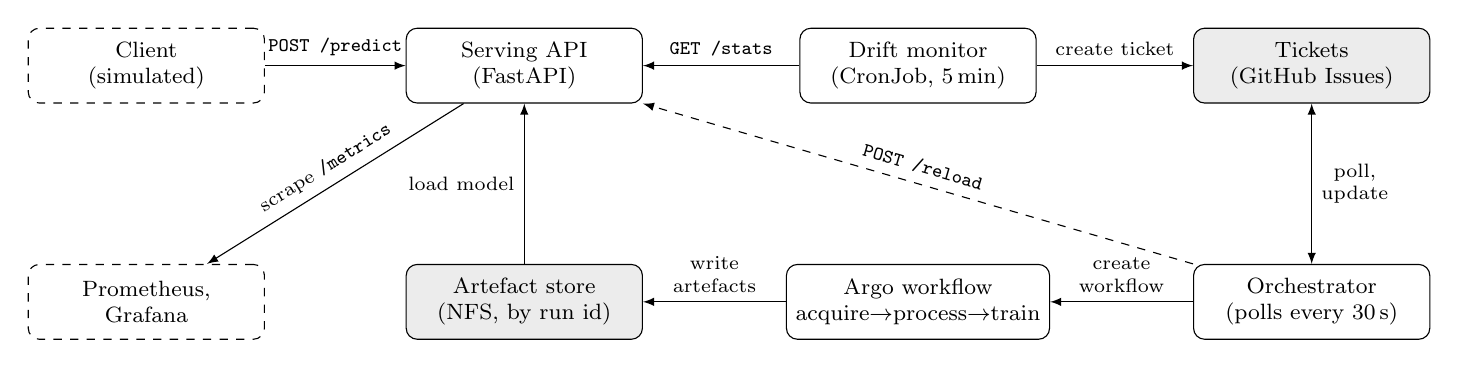
\begin{tikzpicture}[
  box/.style={draw, rounded corners, align=center, minimum height=0.95cm, minimum width=3cm, font=\footnotesize},
  store/.style={box, fill=gray!15},
  ext/.style={box, dashed},
  lbl/.style={font=\scriptsize, align=center}
]
\node[ext]   (client) at (-4.8,0)  {Client\\(simulated)};
\node[box]   (api)    at (0,0)     {Serving API\\(FastAPI)};
\node[box]   (mon)    at (5,0)     {Drift monitor\\(CronJob, 5\,min)};
\node[store] (tix)    at (10,0)    {Tickets\\(GitHub Issues)};
\node[ext]   (obs)    at (-4.8,-3) {Prometheus,\\Grafana};
\node[store] (art)    at (0,-3)    {Artefact store\\(NFS, by run id)};
\node[box]   (wf)     at (5,-3)    {Argo workflow\\acquire$\to$process$\to$train};
\node[box]   (orch)   at (10,-3)   {Orchestrator\\(polls every 30\,s)};

\draw[-latex] (client) -- node[above, lbl]{\texttt{POST /predict}} (api);
\draw[-latex] (mon)    -- node[above, lbl]{\texttt{GET /stats}} (api);
\draw[-latex] (mon)    -- node[above, lbl]{create ticket} (tix);
\draw[latex-latex] (tix) -- node[right, lbl]{poll,\\update} (orch);
\draw[-latex] (orch)   -- node[above, lbl]{create\\workflow} (wf);
\draw[-latex] (wf)     -- node[above, lbl]{write\\artefacts} (art);
\draw[-latex] (art)    -- node[left, lbl]{load model} (api);
\draw[-latex, dashed] (orch.north west) -- node[above, sloped, lbl]{\texttt{POST /reload}} (api.south east);
\draw[-latex] (api)    -- node[above, sloped, lbl]{scrape \texttt{/metrics}} (obs);
\end{tikzpicture}}
\caption{Architecture of the PoC. The monitor also reads the reference statistics from the artefact store and pushes its metrics to a Pushgateway (not drawn).}
\label{fig:poc-arch}
\end{figure}

\subsection{Experimental scenario}

The scenario script runs five steps against the live cluster and logs each of them with a timestamp:
(1)~run the baseline workflow (run identifier \texttt{baseline-001}, no shift) and reload the API;
(2)~send 200 \texttt{/predict} requests drawn from the reference distribution and check that no drift is reported;
(3)~send 200 requests whose six features are shifted by 1.5 reference standard deviations and wait for the monitor to create a ticket;
(4)~wait for the orchestrator to retrain, close the ticket and for the API to serve the new model;
(5)~send the shifted data again and check that the new model's reference no longer reports drift.

The drift rule follows the paper's idea of a runtime check, with parameters we chose: for each feature, $z = |\bar{x}_{\text{now}} - \mu_{\text{ref}}| / \sigma_{\text{ref}}$, where $\bar{x}_{\text{now}}$ is the mean over the last 200 requests; drift is declared when at least three features have $z > 1.0$ and the window holds at least 100 requests.
The monitor runs every five minutes and the orchestrator polls the tickets every 30 seconds.
Retraining uses a shift of 1.5 standard deviations, so the new reference matches the shifted data.

\subsection{Results}

Table~\ref{tab:poc-results} reports the run; every value can be traced to the log file \texttt{scenario/logs/20261015T121211Z.md} (start 12:06:20Z, end 12:12:11Z, total 5\,min\,51\,s). All five steps passed.

\begin{table}[t]
\centering
\caption{Result of the end-to-end run (source: \texttt{scenario/logs/20261015T121211Z.md}).}
\label{tab:poc-results}
\small
\begin{tabularx}{\textwidth}{@{}c >{\raggedright\arraybackslash}p{4.2cm} X l@{}}
\toprule
Step & Expectation & Observation & Outcome \\
\midrule
1 & Baseline workflow succeeds; served model is \texttt{baseline-001} & Workflow succeeded; \texttt{/reload} switched \texttt{issue-6} to \texttt{baseline-001} & Pass \\
2 & $n \geq 100$ and no drift & $n = 200$; largest $z = 0.18$; no feature above 1.0 & Pass \\
3 & \texttt{/stats} shows drift; a \texttt{[drift]} ticket appears & All six features drifted; ticket \#7 created at 12:10:34Z & Pass \\
4 & Ticket closed with label \texttt{done}; served model is \texttt{issue-}\emph{n} & Ticket \#7 closed at 12:12:01Z with labels \texttt{retrain}, \texttt{done}; served model \texttt{issue-7} & Pass \\
5 & No drift against the new model's reference & Model \texttt{issue-7}; $n = 200$; largest $z = 0.13$; no feature above 1.0 & Pass \\
\bottomrule
\end{tabularx}
\end{table}

\paragraph{Timings.}
The shifted requests were sent at 12:07:53Z. The monitor created ticket \#7 at 12:10:34Z (2\,min\,41\,s later, bounded by the five-minute schedule), and the ticket was closed with the new model serving at 12:12:01Z (1\,min\,27\,s after creation). From shifted data to new model took 4\,min\,8\,s.
Across the whole experiment, five ticket-triggered retraining workflows (tickets \#3 to \#7) succeeded, each in 60 to 81 seconds; tickets \#5 and \#7 were created automatically by the monitor, tickets \#3, \#4 and \#6 by hand to test the orchestrator.

\paragraph{Drift evidence.}
At detection, the per-feature $z$ values written in ticket \#7 were 1.44, 1.58, 1.45, 1.46, 1.61 and 1.35 for features \texttt{f0} to \texttt{f5}. After the retraining, the same shifted data gave $z \leq 0.13$ (Table~\ref{tab:poc-results}, step~5). Figure~\ref{fig:poc-grafana} shows the corresponding Grafana dashboard: two drift episodes (largest $z$ about 2.1 and 1.6, six features above the threshold) followed by a return close to zero. Figure~\ref{fig:poc-issue} shows ticket \#7 and Fig.~\ref{fig:poc-argo} the retraining workflow.

\begin{figure}[t]
\centering
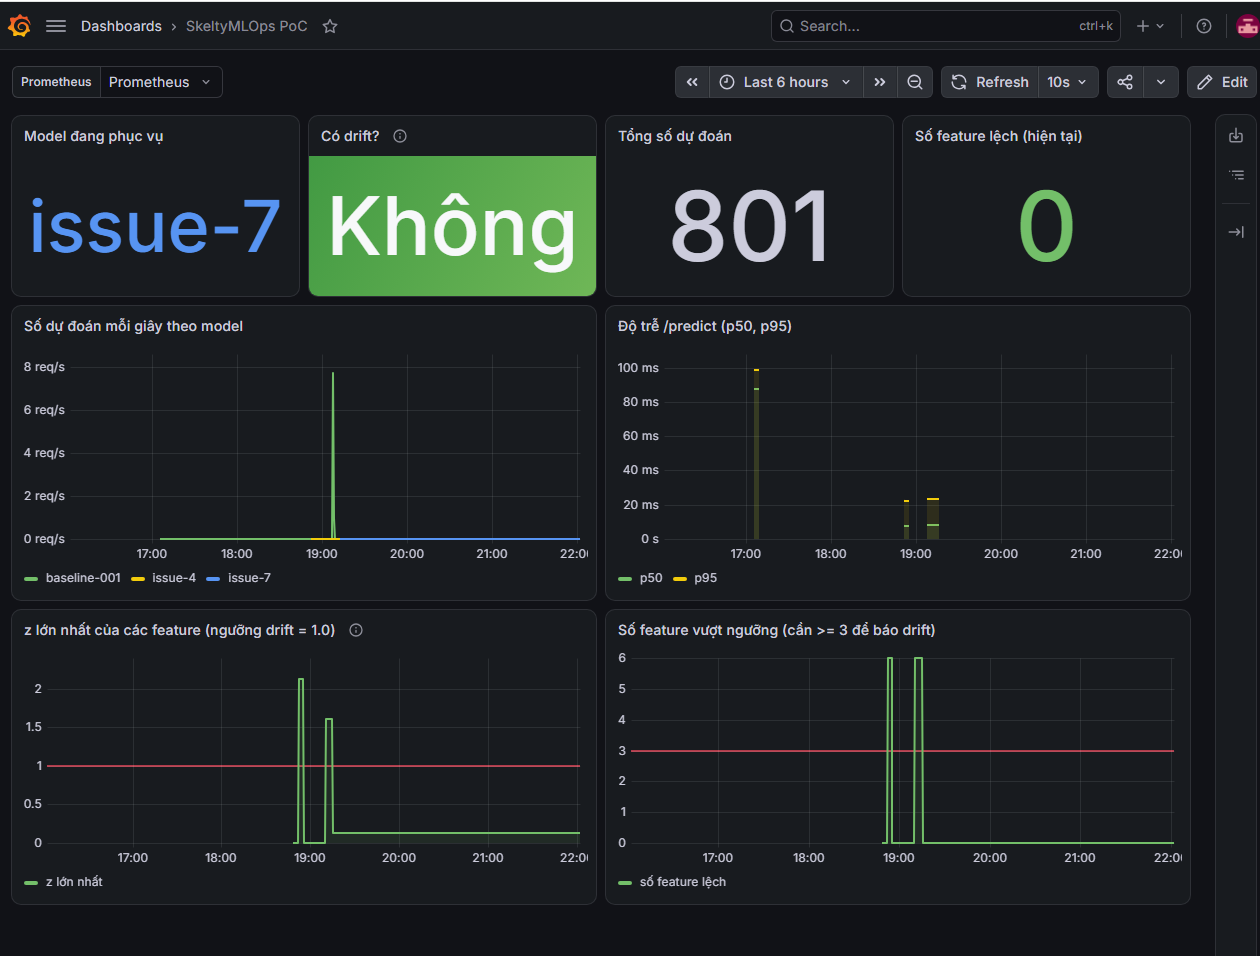
\includegraphics[width=\textwidth]{figures/poc-grafana-6h.png}
\caption{Grafana dashboard over six hours. Top row: served model, drift flag, total predictions, number of drifted features. Middle row: predictions per second by model, prediction latency (p50, p95). Bottom row: largest $z$ with the drift threshold 1.0, and number of drifted features with the threshold 3. Panel titles are in Vietnamese.}
\label{fig:poc-grafana}
\end{figure}

\begin{figure}[t]
\centering
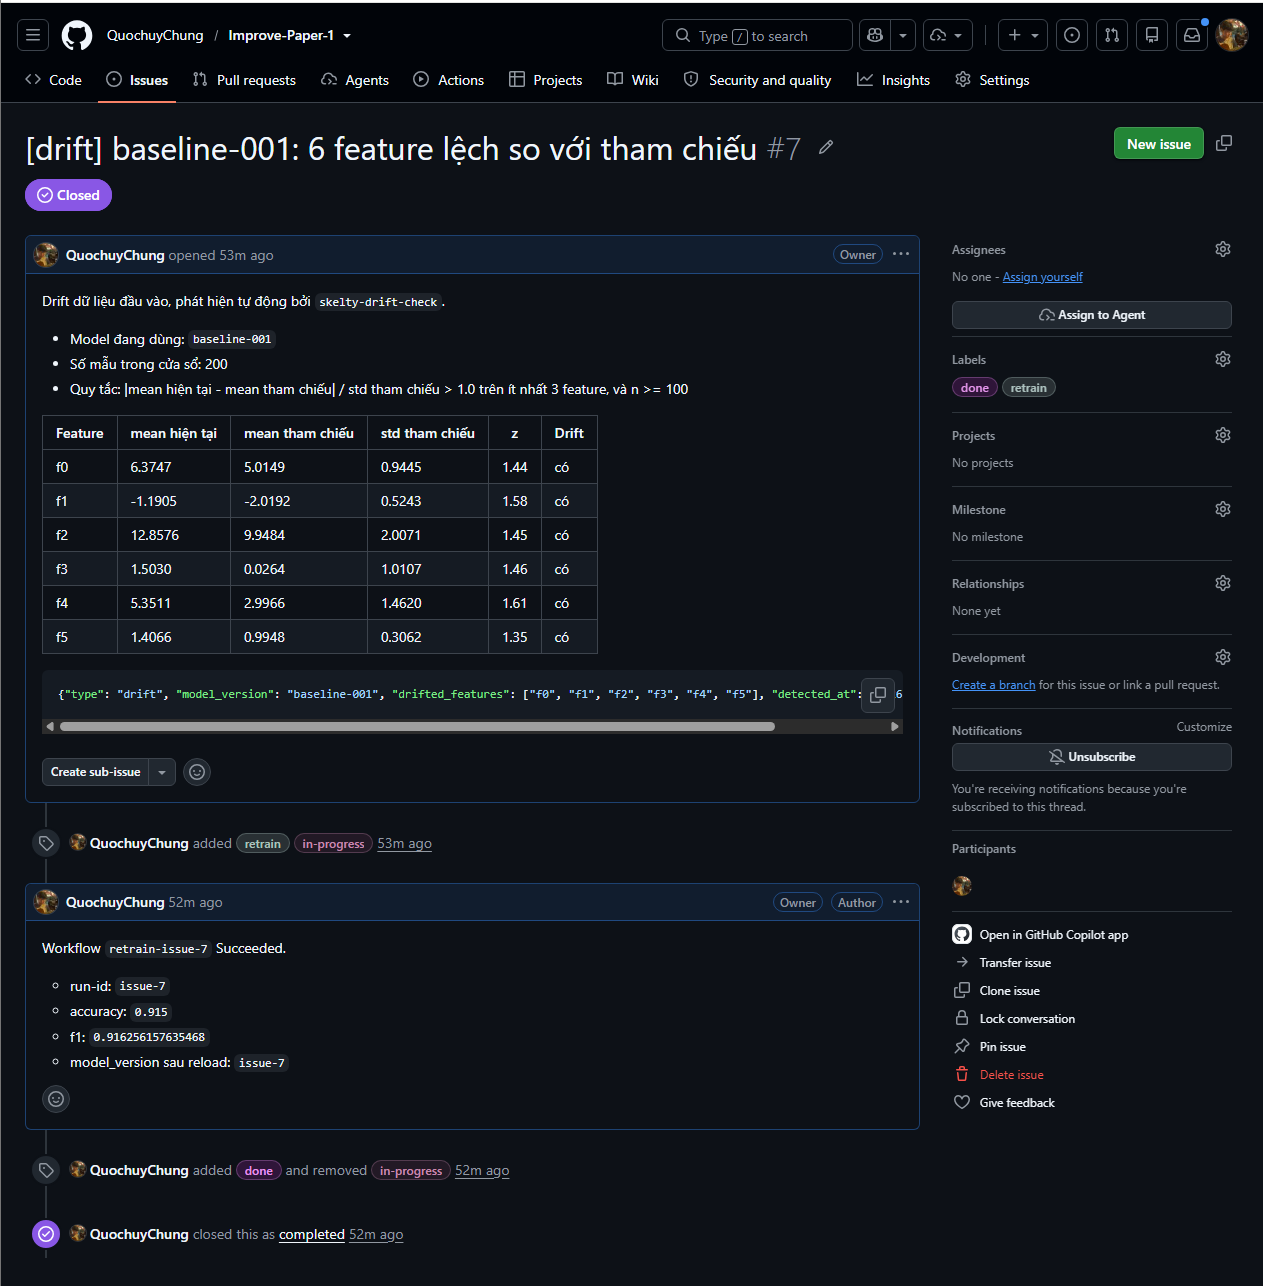
\includegraphics[width=0.85\textwidth]{figures/poc-issue7-auto.png}
\caption{Ticket \#7, created by the drift monitor and closed by the orchestrator. The text (in Vietnamese) states that the drift was detected automatically by the monitor and lists the per-feature statistics; the second comment, written by the orchestrator, gives the run identifier, accuracy, F1 and the model version after the reload. The account name shown is that of the access token shared by both components.}
\label{fig:poc-issue}
\end{figure}

\begin{figure}[t]
\centering
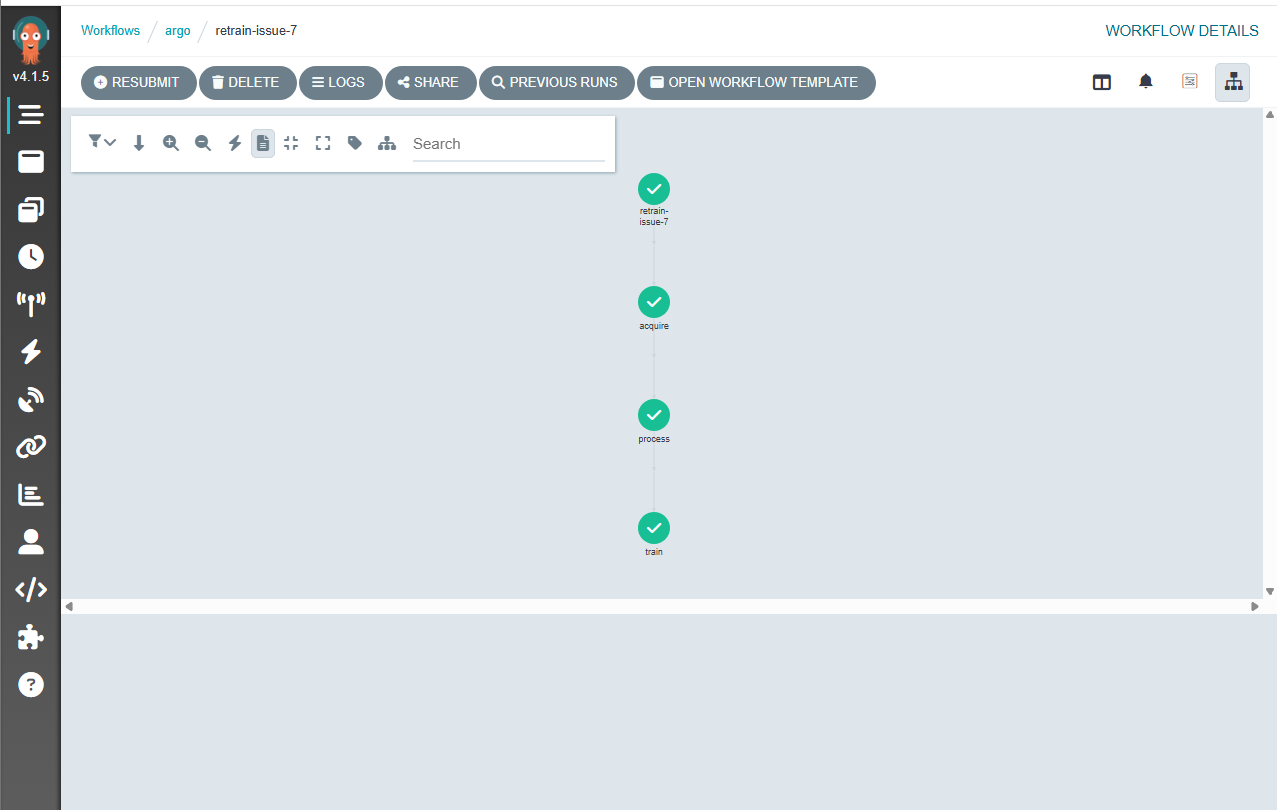
\includegraphics[width=0.7\textwidth]{figures/poc-argo-retrain7.png}
\caption{Argo workflow \texttt{retrain-issue-7}: the three steps \texttt{acquire}, \texttt{process} and \texttt{train} completed successfully.}
\label{fig:poc-argo}
\end{figure}

Accuracy and F1 were identical for the baseline and the retrained models (0.915 and 0.916). This is a property of our synthetic data, where the shift translates the whole problem, and not evidence that retraining is useless; we therefore use the disappearance of the drift, not the accuracy, as the evidence for the loop.

\subsection{Observations relevant to the paper's design}

\begin{itemize}
  \item \textbf{Duplicate tickets.} The monitor creates a ticket only if no open ticket labelled \texttt{retrain} exists. Drift persists until the new model is loaded, so without such a rule each five-minute run would open another ticket. This serialises tickets rather than resolving their interaction, a minimal answer to the concurrent-ticket gap that the paper lists.
  \item \textbf{Actor attribution.} The monitor and the orchestrator used one access token, so GitHub attributes every action to the same account. The timeline shows what happened and when, but not which component acted, whereas the paper's audit trail records the acting actor.
  \item \textbf{Detection latency.} Latency has two components: the five-minute schedule and the sliding window. In a local test, 60 shifted requests mixed with 140 earlier ones gave $z$ between 0.3 and 0.6, below the threshold; with a shift of 1.5 standard deviations, roughly two thirds of the window must be shifted before the rule fires.
  \item \textbf{Event versus ticket.} In the paper a component emits an event and the MPO creates the ticket; in the PoC the monitor creates the ticket itself. This removes one hop but also the MPO's role as the single mediator.
  \item \textbf{Idempotence.} Workflow names derive from the ticket number, so a restarted orchestrator finds the existing workflow instead of creating a second one. This was checked with unit tests using fake clients; we did not restart the orchestrator during the live run.
  \item \textbf{Infrastructure.} During installation the control-plane node became unresponsive because the Kubernetes API server exhausted the node's 3.8\,GiB of memory. No instability was observed during the final run, but resource usage was not recorded.
\end{itemize}

\subsection{Differences from the paper and limitations}
\label{sec:poc-diff}

\begin{itemize}
  \item \textbf{No coordination contracts.} The ticket flow is hard-coded; there is no BPMN process and no contract versioning.
  \item \textbf{No human gates.} The plan approval of the paper's scenario (Step~3) is automatic.
  \item \textbf{Collapsed handoffs.} Dataset update and retraining (Steps~4 and~5) run as one workflow under one actor. Step~6 (code update) is never needed because the feature set is fixed; this corresponds to the ``else'' branch of Algorithm~1, but no gate evaluates the input schema.
  \item \textbf{Storage and versioning.} Files and SHA-256 hashes replace MLflow and DVC, which the authors say their own implementation orchestrates; run identifiers replace names such as \texttt{dataset-v3} and \texttt{model-v2.1}; the code version is not recorded in the manifests.
  \item \textbf{Data and model.} Synthetic data and a simple model.
  \item \textbf{One run.} The scenario was executed once, so no variance is available.
  \item \textbf{Scale.} One small cluster, no load or failure testing; this is not a production setting.
\end{itemize}

\subsection{Summary}

The PoC shows that the drift-to-redeployment loop of the paper's scenario can be assembled from off-the-shelf tools and closes in a few minutes on a small cluster, with evidence traceable to a log and to the tickets. It exercises the feedback loop but deliberately omits the coordination contracts, human gates and multi-actor handoffs that distinguish SkeltyMLOps; the claim about coordination therefore remains untested, and the production gap stated by the authors remains open.
